%\def\Endlec#1{{\Large End Lec #1}}
\graphicspath{{notes/3series/asy/}}

\thispagestyle{empty}


\setcounter{subsection}{12}
\subsection{Some Topological Concepts in Metric Spaces --- non-examinable}

Much of what we have already done is easily transferable to \emph{metric spaces}: these are sets with a suitable notion of \emph{distance.}

\begin{defn}
A \emph{metric} $d$ on a set $S$ is a function $d:S\times S\to\R$ satisfying:
\begin{enumerate}
  \item $d(x,y)\ge 0$ with equality iff $x=y$
  \item $d(x,y)=d(y,x)$
  \item $d(x,z)\le d(x,y)+d(y,z)$ \ ($\triangle$-inequality)
\end{enumerate}
A \emph{metric space} is a set $S$ together with a metric.\\
A sequence $(s_n)$ in a metric space \emph{converges} to $s\in S$ if:
\[\forall \epsilon>0,\ \exists N \text{ such that }n>N\implies d(s_n,s)<\epsilon\]
Similarly, a sequence is \emph{Cauchy} if:
\[\forall \epsilon>0,\ \exists N \text{ such that }m,n>N\implies d(s_m,s_n)<\epsilon\]
\end{defn}

Everything we've done so far has been using the `standard' metric $d(x,y)=\nm{x-y}$ on the set $S=\R$. There are many other options, especially when one has multiple dimensions or even curved spaces. 

\paragraph{Examples}
\begin{enumerate}
  \item On the vector space $\R^n$ we can define infinitely many metrics: for each real $p\ge 1$, let
  \[d_p(x,y)=\left[\sum\limits_{i=1}^n\nm{x_i-y_i}^p\right]^{1/p}\]
  Proving that this satisfies the triangle-inequality for any $p$ is a bit of work! The $d_2$-metric is precisely the `standard' Euclidean metric:
  \[d_2(x,y)=\sqrt{\sum\limits_{i=1}^n(x_i-y_i)^2}\]
  A related metric is
  \[d_\infty(x,y)=\max\left\{\nm{x_i-y_i}:i=1,\ldots,n\right\}\]
  On the real numbers, all these metrics coincide.
  \item Analogously, if $[a,b]$ is an interval, we can define the metrics
  \begin{gather*}
  d_n(f,g)=\left[\int_a^b\nm{f(x)-g(x)}^p\,\dx\right]^{1/p},\qquad
  d_\infty(f,g)=\sup\left\{\nm{f(x)-g(x)}:x\in[a,b]\right\}
  \end{gather*}
  on the set of continuous functions $[a,b]\to\R$.
  \item On any set $S$ one can define the \emph{discrete metric} $d(x,y)=\begin{cases}
  0&\text{ if $x=y$}\\
  1&\text{ if $x\neq y$}
  \end{cases}$
\end{enumerate}
There are many, many more metrics on specific sets. What really matters is that we can repeat a large part of our earlier work using an arbitrary metric on a given set. There are some crucial differences however\ldots

\paragraph{Convergence and boundedness}

Both these concepts turn out to be metric-dependent. A sequence can be bounded or convergent with respect to one metric, but not with respect to another.

\begin{defn}
In a metric space $(S,d)$ a sequence $(s_n)$ is \emph{bounded} if
\[\exists x\in S, M\in\R\text{ such that }\forall n,\ d(S_n,x)\le M\]
\end{defn}
For the usual metric on $\R$, we can always assume that $x=0$. For other metrics however, strange things can happen. For example, the sequence
\[(s_n)=(1,2,3,4,5,6,\ldots)\]
is \emph{bounded} in $\R$ with respect to the discrete metric! Indeed, taking $x=1=M=1$ we see that
\[\forall n,\ d(s_n,1)\le 1\]

Convergence is also metric dependent: here are two examples.

\begin{enumerate}
  \item If $d$ is the discrete metric on $S$, then the only convergent sequences are those which are eventually constant. Indeed, if $\lim s_n=s$, take $\epsilon=\frac 12$ to see that
  \[\exists N\text{ such that }n>N\implies d(s_n,s)<\frac 12\implies d(s_n,s)=0\implies s_n=s\]
  In particular, the sequence $s_n=\frac 1n$ is \emph{divergent} in $\R$ with respect to the discrete metric.
  \item Consider the sequence of continuous functions $(f_n)$ on $[0,1]$ defined by $f_n(x)=x^n$. With respect to the metric $d_2$ we see that
	\[d_2(f_n,0)=\sqrt{\int_0^1x^{2n}\,\dx}=\frac 1{\sqrt{2n+1}}\to 0\]
	whence $f_n$ converges to the zero function on $[0,1]$.\\
	\emph{Pointwise}, however, we evaluate $f_n(x)$ first, and then take the limit: we should obtain the discontinuous function
	\[f(x)=\lim(f_n(x))=\begin{cases}
	0&\text{ if $x<1$}\\
	1&\text{ if $x=1$}
	\end{cases}\]
	\begin{center}
	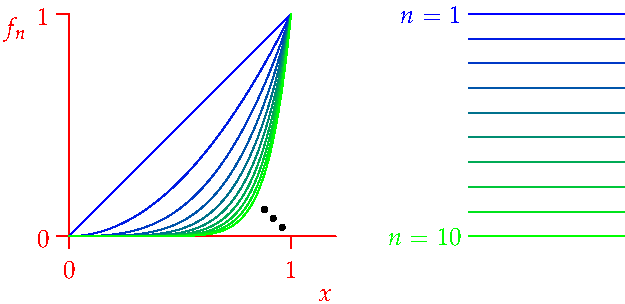
\includegraphics{limfunc}\\
	To what does $(f_n)$ converge?
	\end{center}
	Of course this isn't continuous function, so we cannot claim that $f_n\to f$. If  we consider the infinity-metric, then
	\[d_\infty(f_n,0)=\sup\{x^n:x\in[0,1]\}=1\]
	so that $f_n$ does not converge to $0$: indeed $(f_n)$ is divergent in this metric. In case you're thinking that the discontinuous function $f$ should be the limit, note that, since $f_n(1)=f(1)$ for all $n$, we can write
	\[d_\infty(f_n,f)=\sup\{x^n:x\in[0,1)\}=1\]
	so we \emph{still} have divergence!
\end{enumerate} 

\paragraph{Completeness}

Recalling our discussion of the real numbers (with the usual metric), we now have two competing notions.

\begin{description}
	\item[Least Upper Bound Property] Every non-empty bounded subset has a least upper bound.
	\item[(Cauchy) Completeness] Every Cauchy sequence is convergent. 
\end{description}

We took the least upper bound property as an axiom, and proved completeness. In a general metric space, we don't have a good notion of \emph{ordering}. Partial replacements of the least upper bound property can be found, but we cannot straightforwardly replace the concepts of supremum and infimum. Similarly, monotonicity is no longer a simple idea\footnote{We could, for example, say that a sequence $(s_n)$ is monotone with respect to $s$ if the sequence $d(s_n,s)$ is a monotone sequence of real numbers. Even with this definition, we cannot conclude that bounded monotone sequences converge. For example $s_n=(\cos n,\sin n)$ is divergent in $\R^2$ with the standard metric, yet it is bounded and monotone ($d(s_n,0)=1$ for all $n$).} and many arguments depending on it collapse in a general metric space.\\

Instead, we are forced to rely on the completeness property. First observe that part (a) of Theorem \ref{thm:convcauchy} goes through unmolested:

\begin{lemm}
In any metric space $(S,d)$, convergent sequences are Cauchy.
\end{lemm}

The proof is exactly as before: simply replace $\nm{s_n-s}$ with $d(s_n,s)$, etc. 

\begin{defn}
A metric space $(S,d)$ is \emph{complete} if every Cauchy sequence in $S$ converges to some element $s\in S$.
\end{defn}

\paragraph{Examples}

\begin{enumerate}
  \item We have already seen (Theorem \ref{thm:convcauchy}) that $\R$ is complete with the standard metric. We shall say more below.
  \item Consider the metric $d(x,y)=\nm{e^{-x}-e^{-y}}$ and the sequence $(s_n)=(1,2,3,4,5,\ldots)$ in the metric space $(\R,d)$. This is clearly divergent. However, given $\epsilon>0$, let $N=\max\{1,-\ln\epsilon\}$, then
\[n>m>N\implies d(m,n)=\nm{e^{-m}-e^{-n}}<e^{-m}<e^{-N}\le\epsilon\]
whence $(s_n)$ is Cauchy. Thus $(\R,d)$ is incomplete, even though $\R$ with the standard distance function is complete.
	\item In any set $S$ equipped with the discrete metric, the only Cauchy sequences are those which are eventually constant. These are exactly the same as the convergent sequences, whence we have completeness.
\end{enumerate}

\begin{thm}
$(\R^n,d_p)$ is complete with respect to any of the $p$-metrics, even $p=\infty$.
\end{thm}

\begin{proof}[Sketch Proof]
First observe that, for any $x,y\in\R^n$ and $p\in[0,1)$, we have
\[d_\infty(x,y)\le d_p(x,y)\le d_1(x,y)\le nd_\infty(x,y)\tag*{($\ast$)}\]
Suppose that $(x_k)\subseteq\R^n$ is Cauchy with respect to the $d_\infty$ metric. If $(x^{(i)}_k)\subseteq\R$ is the sequence of $i^\text{th}$ components, then
\[\forall \epsilon>0,\ \exists N\text{ such that }k,l>N\implies \max\left\{\nm{x^{(i)}_k-x^{(i)}_l}:i=1,\ldots,n\right\}<\epsilon\]
In particular, this says that every sequence $(x^{(i)}_k)\subseteq\R$ is Cauchy and thus convergent. It follows that $(x_k)$ converges to some $x\in\R^n$ with respect to $d_\infty$.\\
It should now be clear from ($\ast$) that any sequence which is Cauchy/convergent with respect to $d_\infty$ is also Cauchy/convergent with respect to the other metrics.
\end{proof}

We can similarly prove the Bolzano--Weierstrass theorem for all such metrics on $\R^n$: every bounded sequence has a convergent subsequence. Note however, that Bolzano--Weierstrass \emph{fails} for the discrete metric on $\R$: the `bounded' sequence $(1,2,3,4,5,\ldots)$ has no convergent subsequence.%\\

% When we think about the $d_n$-metrics on spaces of continuous functions, things are more complex. For example, consider the sequence of functions $(f_n)$ in the space $C[0,1]$ defined by
% \[f_n(x)=x^n\]
% If 0 represents the `zero function' ($0:x\mapsto 0$), then we see that
% \[d_2(f_n,0)=\sqrt{\int_0^1x^{2n}\,\dx}=\frac 1{\sqrt{2n-1}}\to 0\]
% If follows that $(f_n)$ is convergent in the space $(C[0,1],d_2)$. Indeed this space can be shown to be complete. However, in the space $(C[0,1],d_\infty)$, we see that
% \[d_\infty(f_n,0)=\sup\{x^n,x\in[0,1]\}=1\]
% for all $n$. The `limit' of the sequence could be thought of as the function
% \[f(x)=\begin{cases}
% 0&\text{ if $x<0$}\\
% 1&\text{ if $x=1$}
% \end{cases}\]
% \emph{But this isn't continuous!} Thus $(C[0,1],d_\infty)$ isn't complete. There are ways to fix such problems, but they would take us too far afield: it is enough to remark that `convergence' is a delicate business in other metric spaces\ldots

\subsubsection*{Open and closed sets}

The study of topology often begins with metric spaces, though these are themselves only special examples of topological spaces. The fundamental building blocks of topology are open sets.

\begin{defn}
A \emph{topological space} is a set $S$ together with a collection of subsets, designated \emph{open,} which satisfy the following properties:
\begin{itemize}
  \item $\emptyset$ and $S$ are both open.
  \item The union of any collection of open sets is open.
  \item The intersection of finitely many open sets is open.
\end{itemize}
\end{defn}

The most familiar example is the set of real numbers: the open sets are precisely unions of open intervals, so that $(-3,2)\cup(4,\infty)$ is open. It is worth thinking about why we are only allowed \emph{finite} intersections: for any $N\in\N$, we see that the finite intersection
\[\bigcup_{n=1}^N\left(-\frac 1n,\frac 1n\right)=\left(-\frac 1N,\frac 1N\right)\]
is an open interval. However,
\[\bigcup_{n=1}^\infty\left(-\frac 1n,\frac 1n\right)=\{0\}\]
is not open.\pagebreak[1]

It is not just the real numbers that form a topological space; \emph{every} metric space is also an example. For this, we have to define open sets relative to a given metric.

\begin{defn}
Let $(S,d)$ be a metric space let $x\in S$ and $r>0$. The \emph{open ball} of radius $r$ centered at $x$ is the set
\[B_r(x):=\{y\in S:d(x,y)<r\}\]
Let $E\subseteq S$. We say that $x\in E$ is \emph{interior} to $E$ if
\[\exists r>0\text{ such that }B_r(x)\subseteq E\]
Write $E^\circ$ for the set of points interior to $E$. We say that $E$ is \emph{open} if $E=E^\circ$.
\end{defn}

\begin{minipage}[t]{0.45\linewidth}\vspace{0pt}
This is a long definition but straightforward in the simple case of $(\R^2,d_2)$. The open ball
\[B_r(x)=\{y\in\R^2:\nm{y-x}<r\}\]
is precisely the disk of radius $r$ centered at $x$, \emph{not including its boundary}. A subset $U\subseteq \R^2$ is open if and only if we can find an open disk subset of $U$ centered at any point of $U$.\\

In the picture are drawn several balls $B_1(0)$ centered at the origin for various values of $p$. The picture helps visualize the inequality $(\ast)$ on the previous page.
\end{minipage}
\begin{minipage}[t]{0.55\linewidth}\vspace{0pt}
\flushright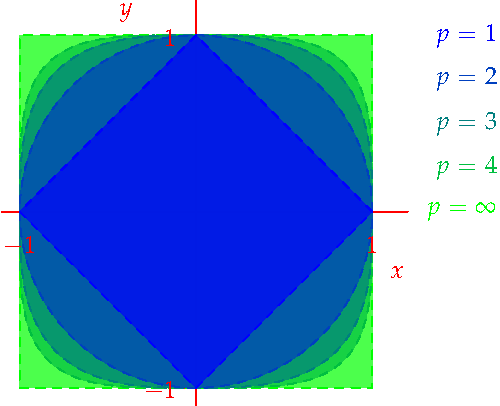
\includegraphics{ball1}
\end{minipage}


\begin{thm}
Every metric space $(S,d)$ is a topological space.
\end{thm}

We need only check the definition: all four parts are essentially trivial.

\begin{proof}
\begin{itemize}
  \item $\emptyset$ is open: there are no points in $\emptyset$ and thus none in its interior!
  \item $S$ is open: let $r$ be any positive value; the open ball $B_r(x)$ is trivially a subset of $S$.
  \item Suppose that $x\in\bigcup U_i$ is a union of open sets. Then $x\in U_i$ for some $i$ and so $\exists B_r(x)\subseteq U_i$. But then $B_r(x)\subseteq\bigcup U_i$, whence the union is also open.
  \item Suppose that $x\in\bigcap\limits_{i=1}^nU_i$ is an intersection of open sets. The $x\in U_i$ for all $i$, whence $\exists r_1,\ldots,r_n>0$ for which
  \[B_{r_i}(x)\subseteq U_i\]
  Let $r=\min\{r_i\}$, then $B_r(x)\subseteq\bigcap U_i$, whence the intersection is open.\hfill\qedhere
\end{itemize}
\end{proof}

\begin{defn}
Let $(S,d)$ be a metric space and $E\subseteq S$. Say that $E$ \emph{closed} if its complement is open.\\
The \emph{closure} of $E$ (written $\cl E$) is the intersection of all closed sets containing $E$.\\
The \emph{boundary} of $E$ is the set $\partial E=\cl E\setminus E^\circ$.
\end{defn}

\begin{thm}
\begin{enumeratea}
	\item $E$ is closed if and only if $E=\cl E$.
	\item $E$ closed if and only if it contains the limit of every convergent sequence of points in $E$.
% 	\item $s\in \cl E$ iff $s$ is the limit of some sequence of points in $E$.
% 	\item $s$ in boundary of $E$ iff belongs to closure of both $E$ and its complement.
\end{enumeratea}
\end{thm}

The proofs are not as important as the observation of how part (b) exactly matches the earlier Definition \ref{defn:closed} of what is meant by a closed set in $\R$ with the usual metric. This illustrates one of the fundamental choices to be made when studying metric spaces: one can take open sets as the basic tool and argue topologically, or one can work with sequences. The choice is often a matter of taste.

\begin{proof}
\begin{enumeratea}
	\item Since $\cl E=\!\!\!\bigcap\limits_{F\text{closed}: E\subseteq F}\!\!\!F$ it is clear that $E\subseteq\cl E$ for any set $E$. Moreover, writing $U=S\setminus F$ for the open complement of the set $F$, we see that
	\[\cl E=\bigcap (S\setminus U)=S\setminus\bigcup U\]
	is itself closed. Thus if $E=\cl E$, we have that $E$ is closed.\\
	Conversely, if $E$ is closed, then $E$ is such a closed set $F$ as described above. But then $\cl E\subseteq E$ and we have equality.
	\item Let $(s_n)\subseteq E$ and suppose that $s_n\to s\in S$ and that $E$ is closed. We want to prove that $s\in E$. Suppose not: then $s$ lies in the open complement $U$ of $E$. But then $\exists r>0$ such that $B_r(s)\subseteq U$. In particular, taking $\epsilon=r$ in the definition of convergence, we obtain a contradiction. Thus $s\in E$.\\
	For the converse, suppose $E$ is not closed. Then its complement $U$ is not open. But then,
	\[\exists s\in U\text{ such that }\forall r>0,\ B_r(s)\not\subseteq U\]
	Taking $r=\frac 1n$, we see that $\exists s_n\in E\cap B_{\frac 1n}(s)$ for each $n$. Otherwise said, $(s_n)$ is a sequence in $E$ which converges to $s\not\in E$.\hfill\qedhere
% 	\item $s\in \cl E$ iff $s$ is the limit of some sequence of points in $E$.
% 	\item $s$ in boundary of $E$ iff belongs to closure of both $E$ and its complement.
\end{enumeratea}
\end{proof}

\subsubsection*{Continuity}

We are about to start considering continuity, though our approach will rely on a metric (indeed the standard metric) on $\R$. The concept is far more general, and illustrate the centrality of open sets to the topological approach.

\begin{defn}
Let $S,T$ be topological spaces. A function $f:S\to T$ is \emph{continuous} if the inverse image $f^{-1}(U)$ of every open set in $T$ is open in $U$.
\end{defn}

Here is an easy example. Take the function $f:\R\to\R:x\mapsto x^2$. One can easily check that, for $a<b$,
\[f^{-1}(a,b)=\begin{cases}
(-\sqrt b,-\sqrt a)\cup(\sqrt a,\sqrt b)&\text{ if $0<a<b$}\\
(-\sqrt b,\sqrt b)&\text{ if $a\le 0<b$}\\
\emptyset&\text{ if $a<b\le 0$}
\end{cases}\]
In all cases the inverse image of an open interval is open. A little thought about how every open set in $\R$ is a union of open intervals show that $f$ is continuous.

% \paragraph{Example}
% The Cantor middle third set: define $I_n$ inductively\\
% $I_0=[0,1]$, $I_1=$ remove middle third, etc. Define $C=\bigcap_{n=0}^\infty I_n$. This is
% \begin{itemize}
%   \item Closed (contains no intervals/interior points)
%   \item Uncountable (more point than rational numbers!)
% \end{itemize} 

